\documentclass{article}
\usepackage[utf8]{inputenc}
\usepackage{hyperref}
\usepackage{listings}
\usepackage{multimedia} % to embed movies in the PDF file
\usepackage{graphicx}
\usepackage{comment}
\usepackage[english]{babel}
\usepackage{amsmath}
\usepackage{amsfonts}
\usepackage{wrapfig}
\usepackage{multirow}
\usepackage{verbatim}
\usepackage{float}
\usepackage{cancel}
\usepackage{caption}
\usepackage{subcaption}
\usepackage{mathdots}
\usepackage{xcolor}
\usepackage{/home/cade/Homework/latex-defs}
\newcommand{\mbf}[1]{\mbox{\boldmath {$#1$}}}

\title{AMATH 573 Homework 4}
\author{Cade Ballew \#2120804}
\date{November 18, 2022}

\begin{document}
	
\maketitle
	
\section{Problem 1}
Consider the Modified Vector Derivative NLS equation
$$
\mbf{B}_t+(\|\mbf{B}\|^2\mbf{B})_x+\gamma (\mbf{e}_1\times
\mbf{B}_0)\left(\mbf{e}_1\cdot (\mbf{B}_x\times
\mbf{B}_0)\right)+\mbf{e}_1\times \mbf{B}_{xx}=0.
$$
where $\mbf{B}=(0,u,v)$, $\mbf{e}_1=(1,0,0)$,
$\mbf{B}_0=(0,B_0,0)$, $\gamma$ is a constant, and the boundary conditions are
$\mbf{B}\rightarrow \mbf{B}_0$, $\mbf{B}_x \rightarrow 0$ as $|x|\rightarrow
\infty$.
\subsection{Part a}
We look for stationary solutions $\mbf{B}=\mbf{B}(z)=\mbf{B}(x-W t)$ by plugging this into our equation via Mathematica. We get that the first entry is identically zero, so we obtain the system of ODEs
\[
\begin{cases}
(-W+3u^2+v^2)u'+2uvv'-v''=0\\
2uvu'+u^2v'-(W+B_0^2\gamma-3v^2)v'+u''=0.
\end{cases}
\]
We can rearrange this and collect terms to get
\[
\begin{cases}
u''=-(u^2v+v^3)'+(W+\gamma B_0^2)v'\\
v''=(uv^2+u^3)'-Wu'.
\end{cases}
\]
Integrating both sides of each equation, we get that
\[
\begin{cases}
u'=-u^2v-v^3+(W+\gamma B_0^2)v+C_1\\
v'=uv^2+u^3-Wu+C_2
\end{cases}
\]
where $C_1,C_2$ are integration constants. Note that these are determined by the boundary conditions which we will plug in at the start of part b. In order for $H(u,v)$ to be a Hamiltonian with canonical Poisson structure, we need that
\[
u'=\pp{H}{v},\quad v'=-\pp{H}{u}.
\]
This of course yields the system
\[
\begin{cases}
	\pp{H}{v}=-u^2v-v^3+(W+\gamma B_0^2)v+C_1\\
	-\pp{H}{u}=uv^2+u^3-Wu+C_2.
\end{cases}
\]
Integrating both sides of each, we get
\[
\begin{cases}
	H(u,v)=-\frac{1}{2} u^2v^2-\frac{v^4}{4}+\frac{1}{2}(W+\gamma B_0^2)v^2+C_1v+c_1(u)\\
	H(u,v)=-\frac{1}{2} u^2v^2-\frac{u^4}{4}+\frac{W}{2}u^2-C_2u+c_2(v).
\end{cases}
\]
Combining these, we get that our system has Hamiltonian given by
\[
H(u,v)=-\frac{1}{2} u^2v^2-\frac{u^4}{4}+\frac{W}{2}u^2-C_2u-\frac{v^4}{4}+\frac{1}{2}(W+\gamma B_0^2)v^2+C_1v,
\]
meaning that our system is Hamiltonian with canonical Poisson structure.

\subsection{Part b}
To find the value of the Hamiltonian such that the boundary conditions are satisfied, we first need to determine $C_1,C_2$ by enforcing the boundary conditions. We do this via the system of equations  
\[
\begin{cases}
	u'=-u^2v-v^3+(W+\gamma B_0^2)v+C_1\\
	v'=uv^2+u^3-Wu+C_2
\end{cases}
\]
from before. As $|x|\to\infty$, we have that $u\to B_0$, $v\to0$, $u'\to0$, $v'\to0$. Plugging this in, we get the system
\[
\begin{cases}
	0=C_1\\
	0=B_0^3-WB_0+C_2
\end{cases}
\]
which can be solved to get that $C_1=0$, $C_2=WB_0-B_0^3$. This means that the value of the Hamiltonian including the boundary conditions is given by
\[
H(u,v)=-\frac{1}{2} u^2v^2-\frac{u^4}{4}+\frac{W}{2}u^2-(WB_0-B_0^3)u-\frac{v^4}{4}+\frac{1}{2}(W+\gamma B_0^2)v^2.
\]
Now, we plug the boundary conditions into our Hamiltonian to get 
\[
H(B_0,0)=-\frac{B_0^4}{4}+\frac{W}{2}B_0^2-(WB_0-B_0^3)B_0=\frac{3}{4}B_0^4-\frac{W}{2}B_0^2.
\]
Setting this constant equal to $H(u,v)$ and defining $U=u/B_0$, $V=v/B_0$, and $W_0=W/B_0^2$ lets us write
\[
\frac{3}{4}B_0^4-\frac{W_0}{2}B_0^4=-\frac{1}{2} B_0^4U^2V^2-B_0^4\frac{U^4}{4}+B_0^4\frac{W_0}{2}U^2-B_0^4(W_0-1)U-B_0^4\frac{V^4}{4}+\frac{1}{2}B_0^4(W_0+\gamma)V^2
\]
which reduces to the curve
\[
\frac{3}{4}-\frac{W_0}{2}=-\frac{1}{2} U^2V^2-\frac{U^4}{4}+\frac{W_0}{2}U^2-(W_0-1)U-\frac{V^4}{4}+\frac{1}{2}(W_0+\gamma)V^2.
\]

\subsection{Part c}
See Mathematica for plots of this curve with $\gamma=1/10$ and $W_0=3$, $W_0=2$, $W_0=1.1$,
$W_0=1$, $W_0=0.95$, $W_0=0.9$ and a discussion of the corresponding solitons. We include crude sketches of the solitons here.\\ \\
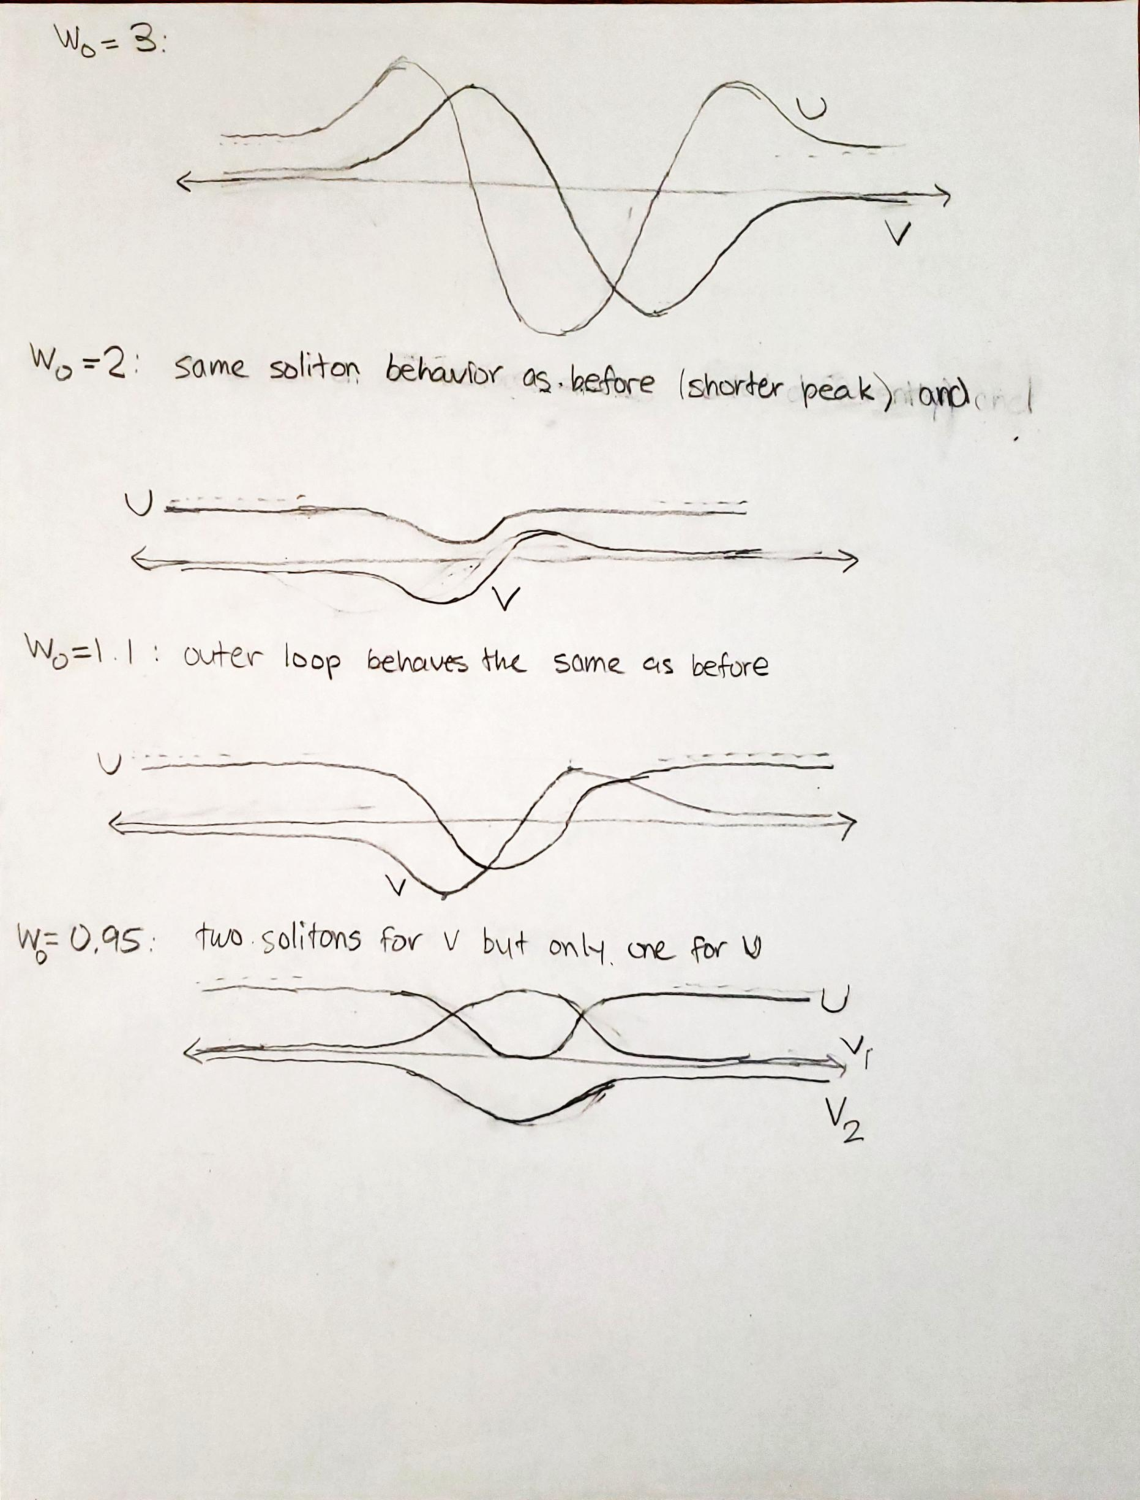
\includegraphics[scale=0.5]{573drawing.pdf}\\

\section{Problem 2}
We wish to show that the canonical Poisson bracket
$$\{f,g\}=\sum_{j=1}^N \left(\pp{f}{q_j}\pp{g}{p_j}-
\pp{f}{p_j}\pp{g}{q_j}\right)
$$
satisfies the Jacobi identity
$$
\{\{f,g\},h\}+\{\{g,h\},f\}+\{\{h,f\},g\}=0.
$$
We do this by brute-force expansion of each term. First,
\begin{align*}
&\{\{f,g\},h\}=\left\{\sum_{j=1}^N \left(\pp{f}{q_j}\pp{g}{p_j}-
\pp{f}{p_j}\pp{g}{q_j}\right),h\right\}\\&=
\sum_{k=1}^N \left(\pp{}{q_k}\left(\sum_{j=1}^N \left(\pp{f}{q_j}\pp{g}{p_j}-
\pp{f}{p_j}\pp{g}{q_j}\right)\right)\pp{h}{p_k}-
\pp{}{p_k}\left(\sum_{j=1}^N \left(\pp{f}{q_j}\pp{g}{p_j}-
\pp{f}{p_j}\pp{g}{q_j}\right)\right)\pp{h}{q_k}\right)\\&=
\sum_{j,k=1}^{N}\left(\ppm{f}{q_j}{q_k}\pp{g}{p_j}\pp{h}{p_k}+\pp{f}{q_j}\ppm{g}{p_j}{q_k}\pp{h}{p_k}-
\ppm{f}{p_j}{q_k}\pp{g}{q_j}\pp{h}{p_k}-\pp{f}{p_j}\ppm{g}{q_j}{q_k}\pp{h}{p_k}\right)\\&+
\sum_{j,k=1}^{N}\left(-\ppm{f}{p_k}{q_j}\pp{g}{p_j}\pp{h}{q_k}-\pp{f}{q_j}\ppm{g}{p_j}{p_k}\pp{h}{q_k}+
\ppm{f}{p_j}{p_k}\pp{g}{q_j}\pp{h}{q_k}+\pp{f}{p_j}\ppm{g}{p_k}{q_j}\pp{h}{q_k}\right).
\end{align*}
Similarly,
\begin{align*}
	&\{\{g,h\},f\}=\sum_{j,k=1}^{N}\left(\ppm{g}{q_j}{q_k}\pp{h}{p_j}\pp{f}{p_k}+\pp{g}{q_j}\ppm{h}{p_j}{q_k}\pp{f}{p_k}-
	\ppm{g}{p_j}{q_k}\pp{h}{q_j}\pp{f}{p_k}-\pp{g}{p_j}\ppm{h}{q_j}{q_k}\pp{f}{p_k}\right)\\&+
	\sum_{j,k=1}^{N}\left(-\ppm{g}{p_k}{q_j}\pp{h}{p_j}\pp{f}{q_k}-\pp{g}{q_j}\ppm{h}{p_j}{p_k}\pp{f}{q_k}+
	\ppm{g}{p_j}{p_k}\pp{h}{q_j}\pp{f}{q_k}+\pp{g}{p_j}\ppm{h}{p_k}{q_j}\pp{f}{q_k}\right),
\end{align*}
and
\begin{align*}
&\{\{h,f\},g\}=\sum_{j,k=1}^{N}\left(\ppm{h}{q_j}{q_k}\pp{f}{p_j}\pp{g}{p_k}+\pp{h}{q_j}\ppm{f}{p_j}{q_k}\pp{g}{p_k}-
\ppm{h}{p_j}{q_k}\pp{f}{q_j}\pp{g}{p_k}-\pp{h}{p_j}\ppm{f}{q_j}{q_k}\pp{g}{p_k}\right)\\&+
\sum_{j,k=1}^{N}\left(-\ppm{h}{p_k}{q_j}\pp{f}{p_j}\pp{g}{q_k}-\pp{h}{q_j}\ppm{f}{p_j}{p_k}\pp{g}{q_k}+
\ppm{h}{p_j}{p_k}\pp{f}{q_j}\pp{g}{q_k}+\pp{h}{p_j}\ppm{f}{p_k}{q_j}\pp{g}{q_k}\right).
\end{align*}
Ordering the terms alphabetically,
\begin{align*}
&\{\{f,g\},h\}+\{\{g,h\},f\}+\{\{h,f\},g\}\\&=
\sum_{j,k=1}^{N}\left(\ppm{f}{q_j}{q_k}\pp{g}{p_j}\pp{h}{p_k}+\pp{f}{q_j}\ppm{g}{p_j}{q_k}\pp{h}{p_k}-
\ppm{f}{p_j}{q_k}\pp{g}{q_j}\pp{h}{p_k}-\pp{f}{p_j}\ppm{g}{q_j}{q_k}\pp{h}{p_k}\right)\\&+
\sum_{j,k=1}^{N}\left(-\ppm{f}{p_k}{q_j}\pp{g}{p_j}\pp{h}{q_k}-\pp{f}{q_j}\ppm{g}{p_j}{p_k}\pp{h}{q_k}+
\ppm{f}{p_j}{p_k}\pp{g}{q_j}\pp{h}{q_k}+\pp{f}{p_j}\ppm{g}{p_k}{q_j}\pp{h}{q_k}\right)\\&+
\sum_{j,k=1}^{N}\left(\pp{f}{p_k}\ppm{g}{q_j}{q_k}\pp{h}{p_j}+\pp{f}{p_k}\pp{g}{q_j}\ppm{h}{p_j}{q_k}-
\pp{f}{p_k}\ppm{g}{p_j}{q_k}\pp{h}{q_j}-\pp{f}{p_k}\pp{g}{p_j}\ppm{h}{q_j}{q_k}\right)\\&+
\sum_{j,k=1}^{N}\left(-\pp{f}{q_k}\ppm{g}{p_k}{q_j}\pp{h}{p_j}-\pp{f}{q_k}\pp{g}{q_j}\ppm{h}{p_j}{p_k}+
\pp{f}{q_k}\ppm{g}{p_j}{p_k}\pp{h}{q_j}+\pp{f}{q_k}\pp{g}{p_j}\ppm{h}{p_k}{q_j}\right)\\&+
\sum_{j,k=1}^{N}\left(\pp{f}{p_j}\pp{g}{p_k}\ppm{h}{q_j}{q_k}+\ppm{f}{p_j}{q_k}\pp{g}{p_k}\pp{h}{q_j}-
\pp{f}{q_j}\pp{g}{p_k}\ppm{h}{p_j}{q_k}-\ppm{f}{q_j}{q_k}\pp{g}{p_k}\pp{h}{p_j}\right)\\&+
\sum_{j,k=1}^{N}\left(-\pp{f}{p_j}\pp{g}{q_k}\ppm{h}{p_k}{q_j}-\ppm{f}{p_j}{p_k}\pp{g}{q_k}\pp{h}{q_j}+
\pp{f}{q_j}\pp{g}{q_k}\ppm{h}{p_j}{p_k}+\ppm{f}{p_k}{q_j}\pp{g}{q_k}\pp{h}{p_j}\right).
\end{align*}
Grouping terms,
\begin{align*}
&\{\{f,g\},h\}+\{\{g,h\},f\}+\{\{h,f\},g\}\\&=
\left(\sum_{j,k=1}^{N}\ppm{f}{q_j}{q_k}\pp{g}{p_j}\pp{h}{p_k}-\sum_{j,k=1}^{N}\ppm{f}{q_j}{q_k}\pp{g}{p_k}\pp{h}{p_j}\right)+\left(\sum_{j,k=1}^{N}\pp{f}{q_j}\ppm{g}{p_j}{q_k}\pp{h}{p_k}-\sum_{j,k=1}^{N}\pp{f}{q_k}\ppm{g}{p_k}{q_j}\pp{h}{p_j}\right)\\&+
\left(\sum_{j,k=1}^{N}\ppm{f}{p_k}{q_j}\pp{g}{q_k}\pp{h}{p_j}-\sum_{j,k=1}^{N}\ppm{f}{p_j}{q_k}\pp{g}{q_j}\pp{h}{p_k}\right)+\left(\sum_{j,k=1}^{N}\pp{f}{p_k}\ppm{g}{q_j}{q_k}\pp{h}{p_j}-\sum_{j,k=1}^{N}\pp{f}{p_j}\ppm{g}{q_j}{q_k}\pp{h}{p_k}\right)\\&+
\left(\sum_{j,k=1}^{N}\ppm{f}{p_j}{q_k}\pp{g}{p_k}\pp{h}{q_j}-\sum_{j,k=1}^{N}\ppm{f}{p_k}{q_j}\pp{g}{p_j}\pp{h}{q_k}\right)+\left(\sum_{j,k=1}^{N}\pp{f}{q_k}\ppm{g}{p_j}{p_k}\pp{h}{q_j}-\sum_{j,k=1}^{N}\pp{f}{q_j}\ppm{g}{p_j}{p_k}\pp{h}{q_k}\right)\\&+
\left(\sum_{j,k=1}^{N}\ppm{f}{p_j}{p_k}\pp{g}{q_j}\pp{h}{q_k}-\sum_{j,k=1}^{N}\ppm{f}{p_j}{p_k}\pp{g}{q_k}\pp{h}{q_j}\right)+\left(\sum_{j,k=1}^{N}\pp{f}{p_j}\ppm{g}{p_k}{q_j}\pp{h}{q_k}-\sum_{j,k=1}^{N}\pp{f}{p_k}\ppm{g}{p_j}{q_k}\pp{h}{q_j}\right)\\&+
\left(\sum_{j,k=1}^{N}\pp{f}{p_k}\pp{g}{q_j}\ppm{h}{p_j}{q_k}-\sum_{j,k=1}^{N}\pp{f}{p_j}\pp{g}{q_k}\ppm{h}{p_k}{q_j}\right)+\left(\sum_{j,k=1}^{N}\pp{f}{p_j}\pp{g}{p_k}\ppm{h}{q_j}{q_k}-\sum_{j,k=1}^{N}\pp{f}{p_k}\pp{g}{p_j}\ppm{h}{q_j}{q_k}\right)\\&+
\left(\sum_{j,k=1}^{N}\pp{f}{q_j}\pp{g}{q_k}\ppm{h}{p_j}{p_k}-\sum_{j,k=1}^{N}\pp{f}{q_k}\pp{g}{q_j}\ppm{h}{p_j}{p_k}\right)+\left(\sum_{j,k=1}^{N}\pp{f}{q_k}\pp{g}{p_j}\ppm{h}{p_k}{q_j}-\sum_{j,k=1}^{N}\pp{f}{q_j}\pp{g}{p_k}\ppm{h}{p_j}{q_k}\right).
\end{align*}
However, each group of terms in parentheses is identically zero. If one switches the dummy index on the second summation in each group $j\to k$, $k\to j$, the first and second sums in each group are identical, meaning that the sums cancel through subtraction. Thus,
$$\{\{f,g\},h\}+\{\{g,h\},f\}+\{\{h,f\},g\}=0
$$ 
as desired.
%\sum_{j,k=1}^{N}\pp{g}{p_j}\left(\ppm{f}{q_j}{q_k}\pp{h}{p_k}-\pp{f}{p_k}\ppm{h}{q_j}{q_k}\right)+\sum_{j,k=1}^{N}\pp{f}{q_j}\left(\ppm{g}{p_j}{q_k}\pp{h}{p_k}-
%\pp{g}{p_k}\ppm{h}{p_j}{q_k}\right)\\&+
%\sum_{j,k=1}^{N}\pp{g}{q_j}\left(\pp{f}{p_k}\ppm{h}{p_j}{q_k}-\ppm{f}{p_j}{q_k}\pp{h}{p_k}\right)+\sum_{j,k=1}^{N}\pp{f}{p_j}\left(\pp{g}{p_k}\ppm{h}{q_j}{q_k}-\ppm{g}{q_j}{q_k}\pp{h}{p_k}\right)\\&+
%\sum_{j,k=1}^{N}\pp{h}{p_j}\left(\pp{f}{p_k}\ppm{g}{q_j}{q_k}-\ppm{f}{q_j}{q_k}\pp{g}{p_k}
%\right)+\sum_{j,k=1}^{N}\pp{h}{q_j}\left(\ppm{f}{p_j}{q_k}\pp{g}{p_k}-\pp{f}{p_k}\ppm{g}{p_j}{q_k}\right)\\&=
%\sum_{j=1}^N\pp{f}{p_j}\left\{\right\}

\section{Problem 3}
We wish to show that the Sine-Gordon equation
$$
u_{tt}-u_{xx}+\sin(u)=0
$$
is Hamiltonian with canonical Poisson structure and Hamiltonian
$$
H=\int \left(\frac{1}{2} p^2+\frac{1}{2}q_{x}^2+1-\cos(q)\right)dx,
$$
where $q=u$, and $p=u_t$. To do this, we simply need to show that 
\[
\pp{q}{t}=\frac{\delta H}{\delta p},\quad\pp{p}{t}=-\frac{\delta H}{\delta q}.
\]
We compute the variational derivatives
\begin{align*}
&\frac{\delta H}{\delta p}=\pp{\mathcal H}{u_t}=u_t,\\
&\frac{\delta H}{\delta q}=\pp{\mathcal H}{u}-\partial_x\pp{\mathcal H}{u_x}=\sin u-\partial_x(u_x)=\sin u-u_{xx}.
\end{align*}
Now, note that
\begin{align*}
&\pp{q}{t}=u_t=\frac{\delta H}{\delta p},\\
&\pp{p}{t}=u_{tt}=u_{xx}-\sin u=-\frac{\delta H}{\delta q},
\end{align*}
so the Sine-Gordon equation is indeed Hamiltonian with canonical Poisson structure and the given Hamiltonian. 

\section{Problem 4}
We wish to check that the conserved quantities $F_{-1}=\int u dx$,
$F_0=\int \frac{1}{2} u^2 dx$,
$F_1=\int\left(\frac{1}{6}u^3-\frac{1}{2}u_x^2\right) dx$, $F_2=\int
\left(\frac{1}{24}u^4-\frac{1}{2}uu_x^2+\frac{3}{10}u_{xx}^2\right)dx$ are
mutually in involution with respect to the Poisson bracket defined by the
Poisson structure given by $\partial_x$. By the antisymmetry of the Poisson bracket, it suffices to check that 
\[
\{F_{-1},F_0\}=\{F_{-1},F_1\}=\{F_{-1},F_2\}=\{F_{0},F_1\}=\{F_{0},F_2\}=\{F_{1},F_2\}=0. 
\]
In the attached Mathematica notebook, we compute each of these and get that this is indeed true.

\section{Problem 5}
To find the fourth conserved quantity of the KdV equation, we assemble the nontrivial weight 8 terms
\[
F_2=\int (a_1u^4+a_2uu_x^2+a_3u_{xx}^2)dx.
\]
Using Mathematica, we compute
\[
\frac{\delta {f_2}_t}{\delta x}=2((12a_1+a_2)u_x^3-2(3a_2+5a_3)u_{xx}u_{xxx}+u_x(3(12a_1+a_2)uu_{xx}-(3a_2+5a_3)u_{xxxx})).
\]
Since we need this to be zero for all $x,t$, we get the linear system
\[
\begin{cases}
12a_1+a_2=0\\
3a_2+5a_3=0.
\end{cases}
\]
If we let $a_1=\frac{1}{24}$, we get that $a_2=-\half$, $a_3=\frac{3}{10}$, meaning that 
\[
F_2=\int
\left(\frac{1}{24}u^4-\frac{1}{2}uu_x^2+\frac{3}{10}u_{xx}^2\right)dx.
\]
Of course, this matches the given $F_2$ from problem 4 as expected.

\section{Problem 6}
Consider a recursion operator $R=B_1
B_0^{-1}$, for the KdV equation with $B_0=\partial_x$ and $B_1=
\partial_{xxx}+\frac{1}{3}(u\partial_x+\partial_x u)$. Using Mathematica, compute that for a given function $v$,
\[
Rv=\frac{2}{3}uv+\frac{1}{3}u_x\int vdx+v_{xx}.
\]
Again using Mathematica, we compute the first KdV flow
\[
u_{t_1}=Ru_x=uu_x+u_{xxx}.
\]
Applying $R$ to this result, we get the second KdV flow up to a rescaling on $t_2$
\[
u_{t_2}=\frac{5}{6}u^2u_x+\frac{10}{3}u_xu_{xx}+\frac{5}{3}uu_{xxx}+u_{xxxxx}.
\]
Applying $R$ again to this result, we get the third KdV equation up to a scaling on $t_3$
\[
u_{t_3}=\frac{35}{54}u^3u_x+\frac{35}{18}u_x^3+\frac{35}{18}u^2u_{xxx}+\frac{35}{3}u_{xx}u_{xxx}+7u_xu_{xxxx}+\frac{7}{9}u(10u_xu_{xx}+3u_{xxxxx})+u_{xxxxxxx}.
\]

\section{Problem 7}
Consider the function $U(x)=2\partial_x^2\ln\left(1+e^{kx+\alpha}\right)$.
We show that for a suitable $k$, $U(x)$ is a solution of the first member of the
stationary KdV hierarchy
$$
6uu_x+u_{xxx}+c_0 u_x=0.
$$
by plugging it in via Mathematica and solving for $c_0$ in terms of $k$. This yields that our function is indeed a solution if $c_0=-k^2$. Now, we let
$u(x,t_1,t_2,t_3,\ldots)=U(x)|_{\alpha=\alpha(t_1,t_2,t_3,\ldots)}$ and determine
the dependence of $\alpha$ on $t_1$, $t_2$ and $t_3$ such that
$u(x,t_1,t_2,t_3,\ldots)$ is simultaneously a solution of the first, second and
third KdV equations
\begin{align*}
u_{t_1}&=6 u u_x+u_{xxx},\\\nonumber
u_{t_2}&=30u^2u_x+20u_x u_{xx}+10u u_{xxx}+u_{5x},\\\nonumber
u_{t_3}&=140 u^3 u_x+70 u_x^3+280 u u_x u_{xx}+70 u_{xx}u_{xxx}+70
u^2 u_{xxx}+42u_x u_{xxxx}+14 u u_{5x}+u_{7x}.
\end{align*}
by plugging it into each via Mathematica and solving for $\alpha$. This yields that
\[
\alpha_{t_1}=k^3\quad\alpha_{t_2}=k^5\quad\alpha_{t_3}=k^7.
\]
Based on this, we guess that
\[
\alpha=\sum_{j=1}^{\infty}k^{2j+1}t_j
\]
yields a one-soliton solution that
solves the entire KdV hierarchy.

\section{Problem 8}
Consider the function
$$
U(x)=2\partial_x^2\ln\left(1+e^{k_1
	x+\alpha}+e^{k2_x+\beta}+\left(\frac{k_1-k_2}{k_1+k_2}\right)^2
e^{k_1x+k_2 x+\alpha+\beta}\right).
$$
We show that for a suitable $k_1$, $k_2$,
$U(x)$ is a solution of the second member of the stationary KdV hierarchy
$$
30u^2u_x+20u_x u_{xx}+10u u_{xxx}+u_{5x}+c_1(6uu_x+u_{xxx})+c_0 u_x=0.
$$
by plugging it into Mathematica and solving for $c_0,c_1$ in terms of $k_1,k_2$. This yields that our function is indeed a solution if 
\[
c_0=k_1^2k_2^2,\quad c_1=-k_1^2-k_2^2.
\]
Now, we let
$u(x,t_1,t_2,t_3,\ldots)=U(x)|_{\alpha=\alpha(t_1,t_2,t_3,\ldots),
	\beta=\beta(t_1,t_2,t_3,\ldots)}$ and determine the dependence of $\alpha$ and $\beta$ on $t_1$, $t_2$ and $t_3$ such that
$u(x,t_1,t_2,t_3,\ldots)$ is simultaneously a solution of the first, second and
third KdV equations by it into each via Mathematica and solving for $\alpha,\beta$.
This yields that
\[
\alpha_{t_1}=k_1^3\quad\alpha_{t_2}=k_1^5\quad\alpha_{t_3}=k_1^7
\]
and 
\[
\beta_{t_1}=k_2^3\quad\beta_{t_2}=k_2^5\quad\beta_{t_3}=k_2^7.
\]
Based on this, we guess that
\[
\alpha=\sum_{j=1}^{\infty}k_1^{2j+1}t_j,\quad\beta=\sum_{j=1}^{\infty}k_2^{2j+1}t_j
\]
yields a two-soliton solution that
solves the entire KdV hierarchy.

\end{document}
